% 
% Annual CCN conference
% Sample LaTeX Two-Page Summary -- Proceedings Format
% based on the prior cognitive science style file

% Original : Ashwin Ram (ashwin@cc.gatech.edu)       04/01/1994
% Modified : Johanna Moore (jmoore@cs.pitt.edu)      03/17/1995
% Modified : David Noelle (noelle@ucsd.edu)          03/15/1996
% Modified : Pat Langley (langley@cs.stanford.edu)   01/26/1997
% Latex2e corrections by Ramin Charles Nakisa        01/28/1997 
% Modified : Tina Eliassi-Rad (eliassi@cs.wisc.edu)  01/31/1998
% Modified : Trisha Yannuzzi (trisha@ircs.upenn.edu) 12/28/1999 (in process)
% Modified : Mary Ellen Foster (M.E.Foster@ed.ac.uk) 12/11/2000
% Modified : Ken Forbus                              01/23/2004
% Modified : Eli M. Silk (esilk@pitt.edu)            05/24/2005
% Modified : Niels Taatgen (taatgen@cmu.edu)        10/24/2006
% Modified : David Noelle (dnoelle@ucmerced.edu)     11/19/2014
% Modified : Konrad Kording (koerding@gmail.com) 2/15/2017

\documentclass[10pt,letterpaper]{article}

\usepackage{ccn}
\usepackage{pslatex}
\usepackage{apacite}
\usepackage{graphicx}

\graphicspath{ {../static/} }

\title{Do convolutional neural networks exhibit human-like attentional effects? 
Conflicting results from a visual search task}
 
\author{{\large \bf David Nicholson (dnicho4@emory.edu)} \\
  A Department, 1234 Example Street\\
A City, State 12345 A country
  \AND {\large \bf Astrid Prinz (AnotherPerson@this.planet.edu)} \\
  A Department, 1234 Example Street\\
A City, State 12345 A country}


\begin{document}

\maketitle


\section{Abstract}
{
\bf
Convolutional neural networks (CNNs) trained to perform tasks such as image classification
with human-like accuracy acquire representations similar to those in the primate 
visual system. Do CNNs that are pre-trained to use such representations conversely exhibit 
human-like behavior? We test this with a visual search task that has long been used to 
investigate attention mechanisms. We first show that CNNs using weights trained for image 
classification can exhibit human-like attentional effects when performing this visual 
search task. However, we then demonstrate that these effects can be 
eliminated, without changing the lower-level learned representations, by modifying other 
parameters of training and the balance of classes in the training data. One explanation 
for this finding is that we are only training networks to discriminate single types of 
visual search stimuli. We further test CNNs trained to perform multiple tasks.
We go on to show that manipulating the 
discriminability of the target and distractors in the task can produce attentional 
effects in spite of the changes we made to training. Based on these results, we conclude 
that CNNs do not show attentional effects.
}
\begin{quote}
\small
\textbf{Keywords:} 
attention;visual search
\end{quote}

\section{Introduction}
\subsection{Attention}
Multiple converging lines of evidence seem to suggest that training neural networks to 
perform tasks with human-like abilities causes them to acquire brain-like representations.

- If brain-like representations are both necessary and sufficient for human-like 
intelligence, then shouldn't the converse also be true? Shouldn't neural networks that 
have acquired brain-like representations behave like humans when asked to perform related 
tasks? We test this 

In these fields, theories of attention mechanisms are often built on 
results produced by experimental manipulations that impair behavior.
Perhaps the pre-eminent example of this approach to understanding attention is a 
a long-established form of visual search task [@wolfeVisualSearch1998]. In this behavioral
paradigm, subjects view a set of discrete items on a flat background and report whether a 
target is present or absent among distractors. Classically, results from this paradigm 
have been used to support different theories of \bf{selective covert visual attention}, 
a term that requires some defintion. The term "selective" is simply supposed to mean 
some mechanism that selects some visual inputs for further processing while necessarily 
discarding others. The word "covert" in this context means any mechanism that occurs 
"centrally", i.e. inside the brain, without overt orientation, i.e. without eye or head 
movements.
- here we do not 

Our goal here is not to resolve the debate about whether selective covert visual 
attention is serial or parallel. Rather our goal is to better understand attention as 
defined in cognitive science and reconcile that with the definition used in artificial 
intelligence.

\subsection{visual search}
\textbf{set size effects}

\begin{figure}[ht]
\begin{center}
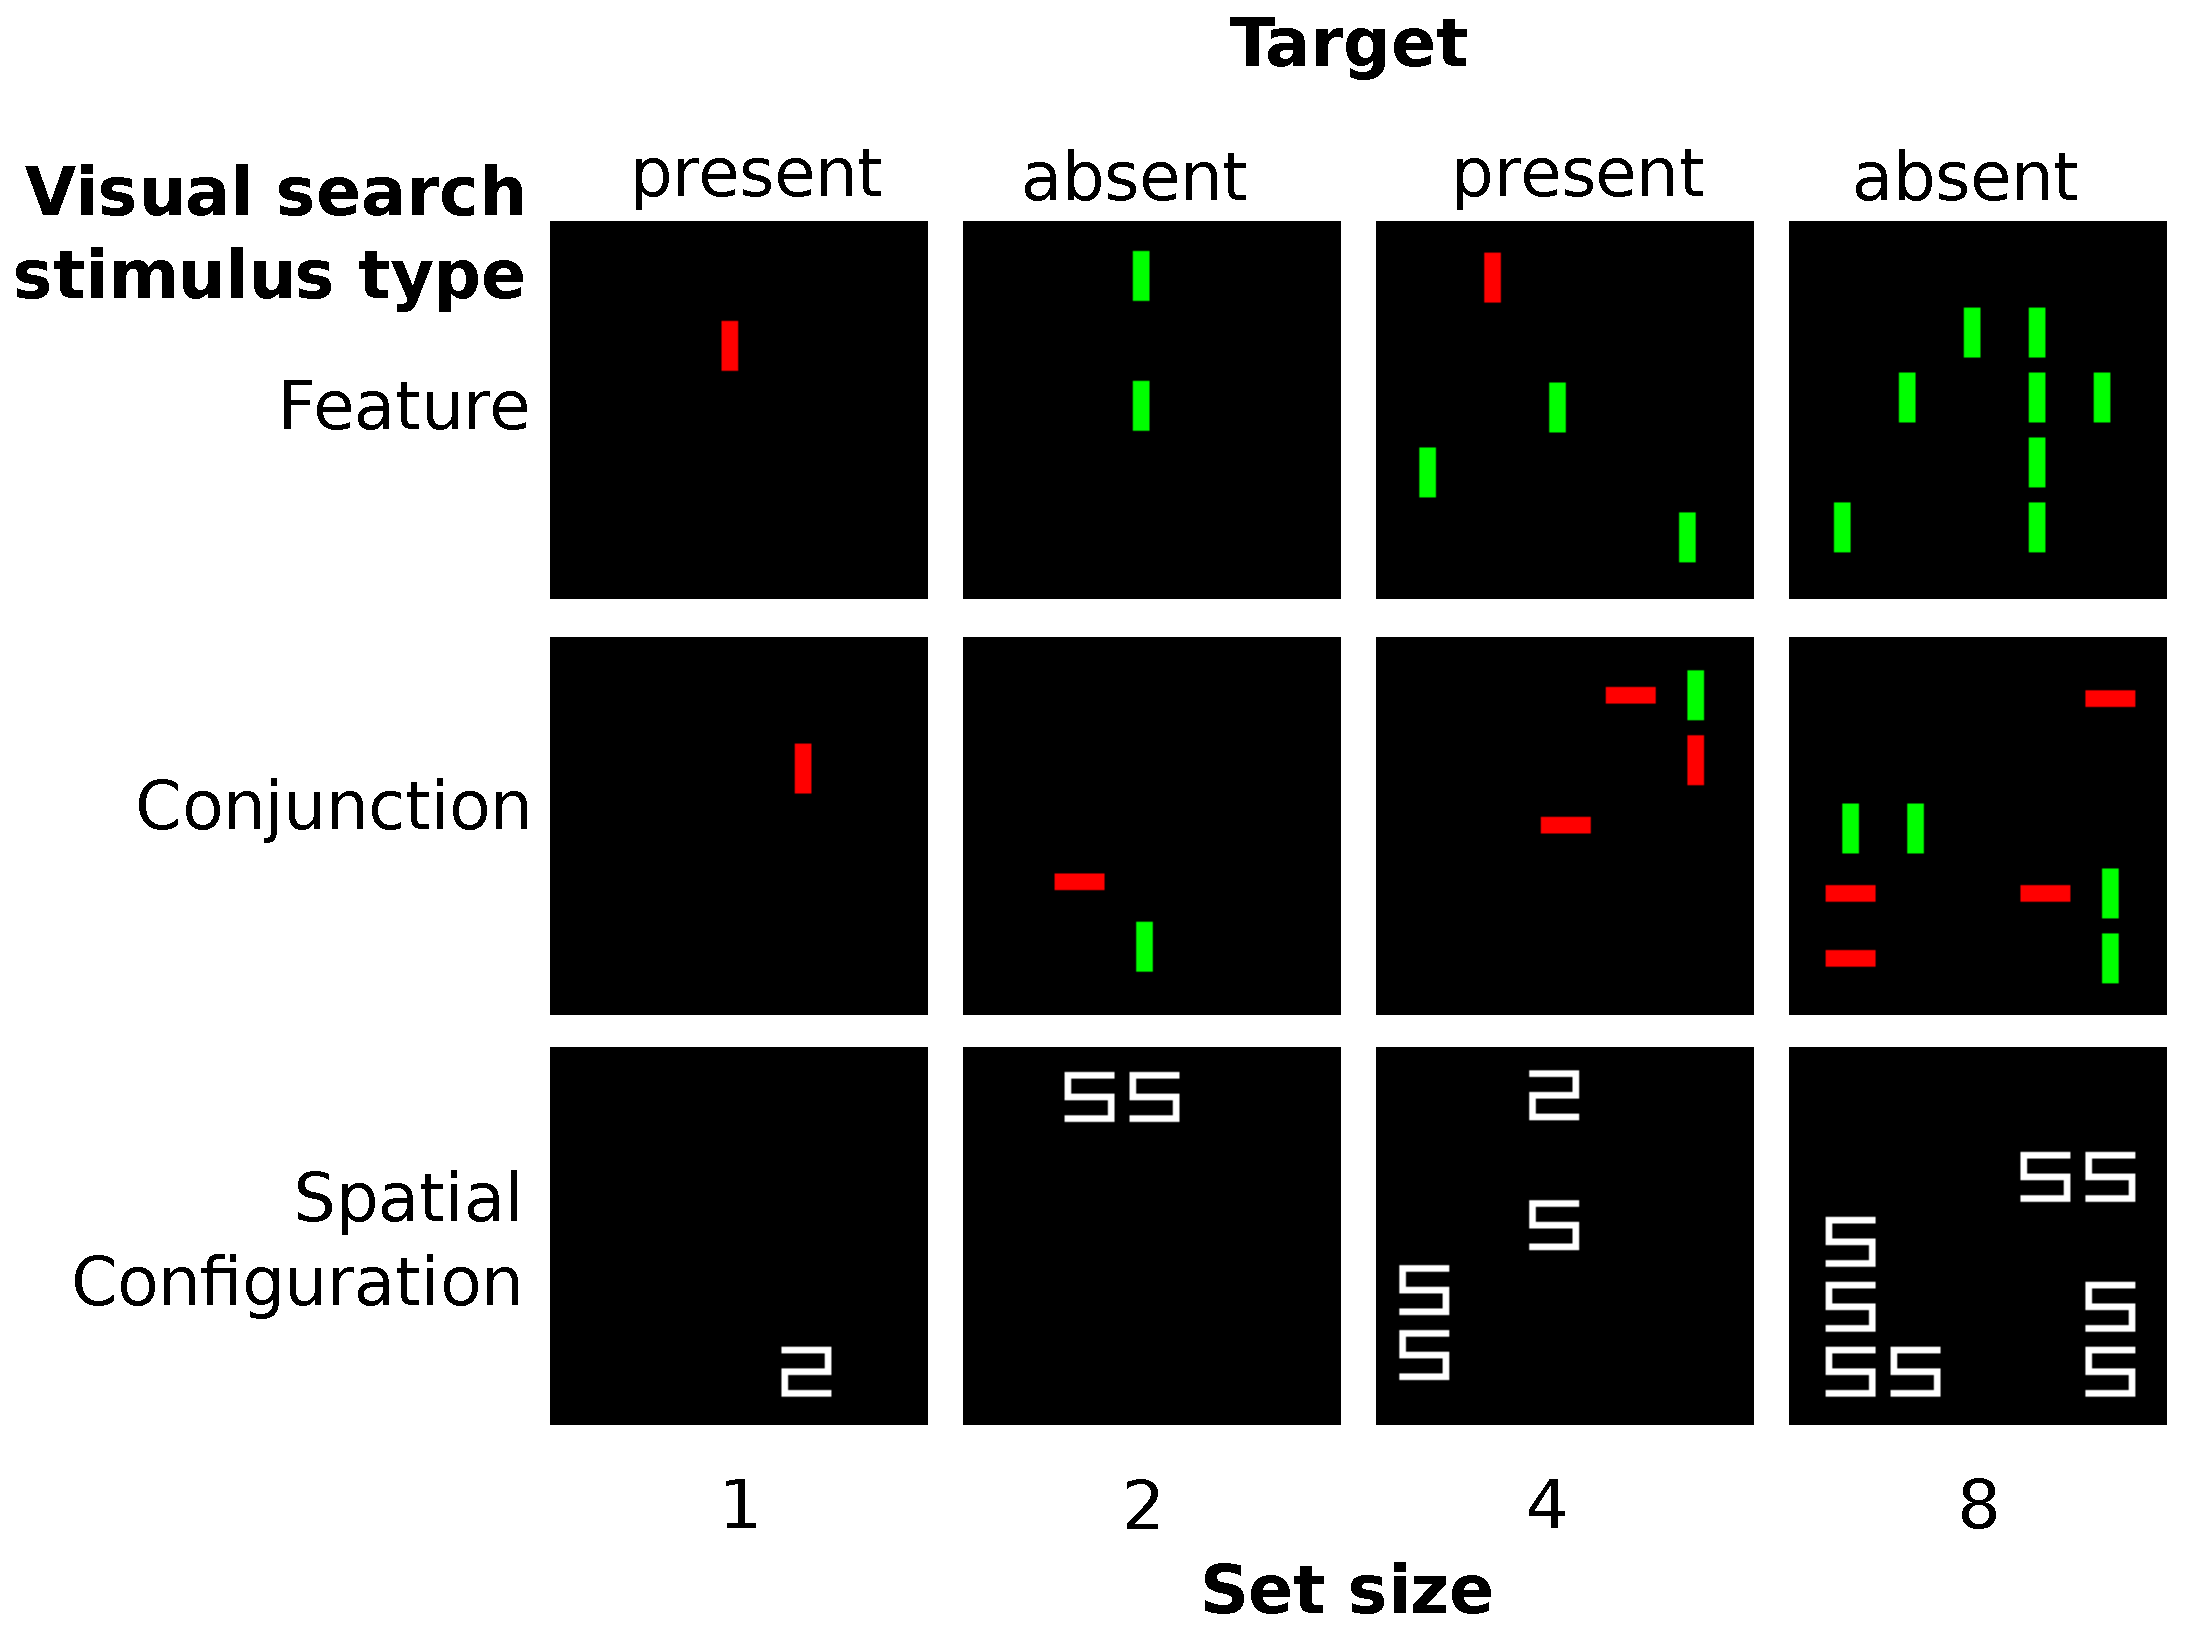
\includegraphics[width=\columnwidth]{fig1/fig1.eps}
\end{center}
\caption{A classic form of visual search task.} 
\label{sample-figure}
\end{figure}



\section{Results}

\subsection{CNNs trained for image classification show set size effects}

\begin{figure}[ht]
\begin{center}
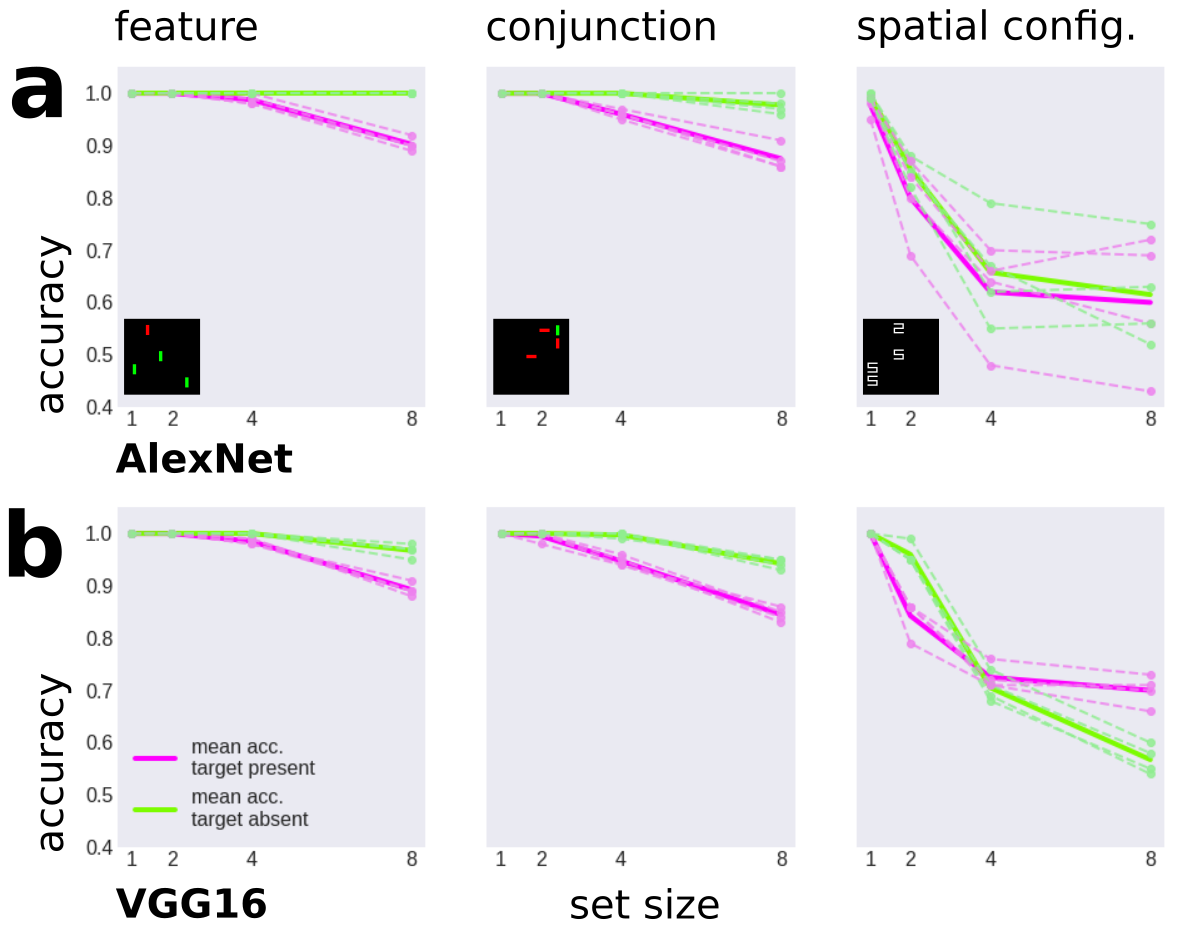
\includegraphics[width=\columnwidth]{fig2/fig2.png}
\end{center}
\caption{CNNs trained for image classification show set size effects.} 
\label{sample-figure}
\end{figure}


\subsection{Changing hyperparameters and balancing the dataset largely 
eliminates set size effects}

Because we defined set size with effects in terms of accuracy, it could 
be the case that our results do not arise because of a similarity between 
how CNNs and brains process images. Instead they could be an artifact of 
how we trained networks. As discussed below, we see this as a general issue 
for studies that compare cognitive science and artificial intelligence, and 
so here we report results that might otherwise be considered methodological 
troubleshooting.
To determine whether our results were an artifact of training, we considered aspects of 
training that can impair accuracy: the amount of training data, the hyperparameters 
used to train the network, and the statistics of the dataset. As shown in 
figure two, we found that all three factors contributed to the effect we saw.
We generated learning curves where we plotted accuracy on the training and 
test set as a function of the training set size. These learning curves revealed 
that the original size we chose for the training set was far from where 
accuracy on training and test set converged. This result indicates that the 
network can improve accuracy with increased training data. To gain insight 
about how accuracy depended on the learning rate, a key hyperparameter, and 
the balance of the data set, we plotted accuracy on the training set 
\emph{separately for each set size in the visual search stimuli}. As shown in 
figure 2b, these plots revealed (1) that accuracy had not yet reached some asymptotic 
value, and (2) that there was an inverse relationship between the set size of 
a visual search stimulus and the rate that its accuracy increased.
To test whether we could improve the learning rate, we used random search, and 
did find we were able to improve accuracy and decrease training time by 
abandoning the fine-tuning approach and instead using a typical learning rate 
on the fully-connected layers (and simply freezing the pre-trained weights in other layers). 

Use standard APA citation format. Citations within the text should
include the author's last name and year. If the authors' names are
included in the sentence, place only the year in parentheses, as in
\citeA{NewellSimon1972a}, but otherwise place the entire reference in
parentheses with the authors and year separated by a comma
\cite{NewellSimon1972a}. List multiple references alphabetically and
separate them by semicolons
\cite{ChalnickBillman1988a,NewellSimon1972a}. Use the
``et~al.'' construction only after listing all the authors to a
publication in an earlier reference and for citations with four or
more authors.

\section{Discussion}

\subsection{Implications for comparative studies of neuroscience and 
artificial intelligence}
- problem for any 

- e.g. Bengio study of gestalt fx

\subsection{Implications for the study of attention in the brain}
- if the task is possible to perform perfectly, who needs attention?
- brain optimized for something else besides classifying static images
- in this sense, consistent with findings that recurrent

\subsection{Footnotes}

Indicate footnotes with a number\footnote{Sample of the first
footnote.} in the text. Place the footnotes in 9~point type at the
bottom of the column on which they appear. Precede the footnote block
with a horizontal rule.\footnote{Sample of the second footnote.}


\subsection{Tables}

Number tables consecutively. Place the table number and title (in
10~point) above the table with one line space above the caption and
one line space below it, as in Table~\ref{sample-table}. You may float
tables to the top or bottom of a column, or set wide tables across
both columns.

\begin{table}[!ht]
\begin{center} 
\caption{Sample table title.} 
\label{sample-table} 
\vskip 0.12in
\begin{tabular}{ll} 
\hline
Error type    &  Example \\
\hline
Take smaller        &   63 - 44 = 21 \\
Always borrow~~~~   &   96 - 42 = 34 \\
0 - N = N           &   70 - 47 = 37 \\
0 - N = 0           &   70 - 47 = 30 \\
\hline
\end{tabular} 
\end{center} 
\end{table}


\subsection{Figures}

Make sure that the artwork can be printed well (e.g. dark colors) and that 
the figures make understanding the paper easy.
 Number figures sequentially, placing the figure
number and caption, in 10~point, after the figure with one line space
above the caption and one line space below it, as in
Figure~\ref{sample-figure}. If necessary, leave extra white space at
the bottom of the page to avoid splitting the figure and figure
caption. You may float figures to the top or bottom of a column, or
set wide figures across both columns.

\begin{figure}[ht]
\begin{center}
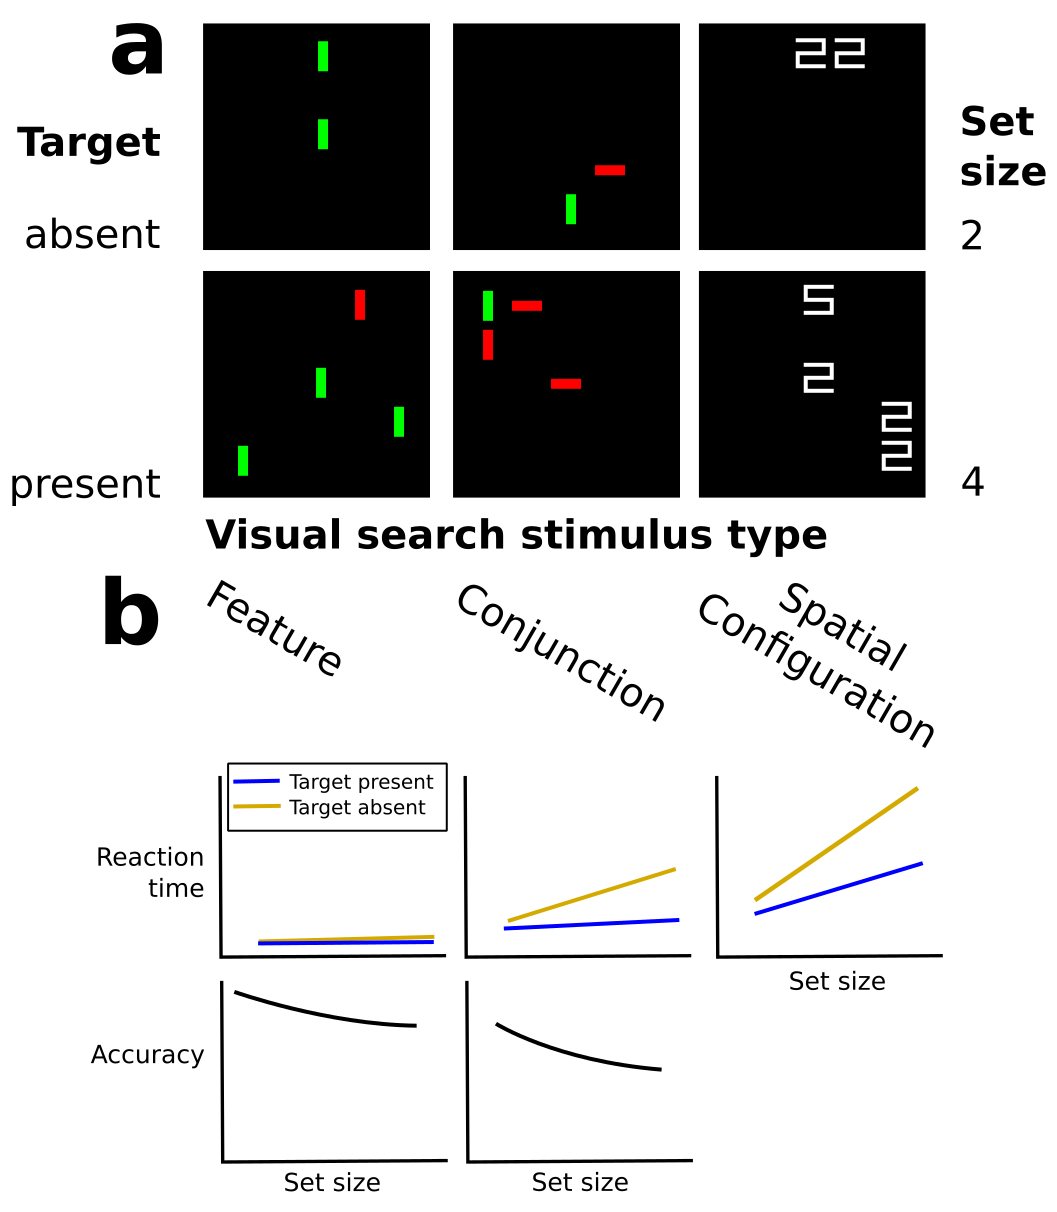
\includegraphics{fig1}
\end{center}
\caption{This is a figure.} 
\label{sample-figure}
\end{figure}


\section{Acknowledgments}

Place acknowledgments (including funding information) in a section at
the end of the paper.


\section{References Instructions}

Follow the APA Publication Manual for citation format, both within the
text and in the reference list, with the following exceptions: (a) do
not cite the page numbers of any book, including chapters in edited
volumes; (b) use the same format for unpublished references as for
published ones. Alphabetize references by the surnames of the authors,
with single author entries preceding multiple author entries. Order
references by the same authors by the year of publication, with the
earliest first.

Use a first level section heading, ``{\bf References}'', as shown
below. Use a hanging indent style, with the first line of the
reference flush against the left margin and subsequent lines indented
by 1/8~inch. Below are example references for a conference paper, book
chapter, journal article, dissertation, book, technical report, and
edited volume, respectively.

\nocite{ChalnickBillman1988a}
\nocite{Feigenbaum1963a}
\nocite{Hill1983a}
\nocite{OhlssonLangley1985a}
% \nocite{Lewis1978a}
\nocite{Matlock2001}
\nocite{NewellSimon1972a}
\nocite{ShragerLangley1990a}


\bibliographystyle{apacite}

\setlength{\bibleftmargin}{.125in}
\setlength{\bibindent}{-\bibleftmargin}

\bibliography{ccn_style}


\end{document}
